% ----------------------------------------------------------


\chapter[Fundamentação Teórica]{Fundamentação Teórica}\label{Fundamentacao}
\begin{enumerate}
   \item  Como contribuição teórica inicial para o nosso projeto, temos o material do canal no Youtube 'Python Engineer' a playlist de vídeo aulas,  'Chat Bot With PyTorch - NLP Beginner Tutorial' \footnote{\url{https://www.youtube.com/playlist?list=PLqnslRFeH2UrFW4AUgn-eY37qOAWQpJyg}}. A partir desse conteúdo poderemos dar início aos nossos desenvolvimentos e pesquisas. No tutorial, é desenvolvido um chatbot simples usando PyTorch e Deep Learning. Também fornecendo uma introdução a algumas técnicas básicas de Processamento de Linguagem Natural (PLN).

   \item Seguiremos, também, os conteúdos já aprendidos nas aulas de  'Inteligência Artifical 2022/2 - UENF' para nos auxiliar na formulação teórica do nosso projeto.

   \item  Salientamos que com o decorrer do projeto nossas referências de materiais, para esse projeto, tenderá a aumentar devido a novas descobertas.
\end{enumerate}







\chapter[Metodologia]{Metodologia}

Baseado no “Project-based learning” \cite{krajcik2006project}. Seguiremos os estudos através de um projeto que aborda problemas do mundo real, cujo muitos não tem resposta única. Ao longo desse projeto será possível fazer novas perguntas e encontrar suas possíveis respostas por meio de uma investigação sustentada.

\justifying
\vspace {1mm}

Este Plano de Pesquisa também utilizará as seguintes metodologias:
\begin{itemize}
   \item \textit{Pesquisa Exploratória; visando promover o enriquecimento do conhecimento sobre os diferentes assuntos relacionados a IA, ML, e Chatbots:
         }
         \begin{itemize}
            \item \textit{Levantamento Bibliográfico;}
            \item \textit{Levantamento documental;}
            \item \textit{Minicursos e Vídeo aulas;}
            \item \textit{Obtenção de experiências.}
         \end{itemize}
\end{itemize}

\chapter[Construindo um Chatbot com Pytorch]{Construindo um Chatbot com Pytorch}

Já pensou em como Alexa, Siri ou assistente de voz do Google funcionavam? Neste capítulo daremos início à construção de um chatbot para interação com usuários de uma loja virtual.

Antes de continuar, abaixo encontra-se a lista de requisitos para o nosso projeto:
\justifying
\begin{itemize}
   \item \textit{Python 3}
   \item \textit{Dictionaries e Lists}
   \item \textit{Numpy}
   \item \textit{Pandas}
   \item \textit{Pytorch}
   \item \textit{Natural Language Processing (Bag of Words)}

\end{itemize}

\section[Importando Bibliotecas Relevantes]{Importando Bibliotecas Relevantes}
\begin{lstlisting}[language=Python, caption=Python Bibliotecas]

   import numpy as np
   import random
   import json
   import nltk
   import torch
   import torch.nn as nn
   from torch.utils.data import Dataset, DataLoader
\end{lstlisting}


\section[Criando funções personalizadas]{Criando funções personalizadas}
Criaremos funções personalizadas para que seja fácil implementá-las posteriormente.
\justifying
\begin{lstlisting}[language=Python, caption=Python Funções personalizadas]
def tokenize(sentence):
    return nltk.word_tokenize(sentence)

def stem(word):
    return stemmer.stem(word.lower())

\end{lstlisting}
Nltk ou kit de ferramentas de linguagem natural é uma biblioteca realmente útil que contém classes importantes que serão úteis em qualquer uma de suas tarefas de PNL.
\justifying
\section[Stemming]{Stemming}


Se tivermos as seguintes palavras como Andei, Ande, Andarei, Andamento, Andando, Andante, podem parecer palavras diferentes, mas geralmente têm o mesmo significado e também a mesma forma base; "and".
O processo de stemização (do inglês, stemming) consiste em reduzir uma palavra ao seu radical. A palavra “meninas” se reduziria a “menin”, assim como “meninos” e “menininhos”. As palavras “gato”, “gata”, “gatos” e “gatas” reduziriam-se para “gat” \footnote{\url{https://www.computersciencemaster.com.br/como-reduzir-uma-palavra-ao-seu-radical-em-python-stemming/}}.
Então, para que nosso modelo entenda todas as formas diferentes das mesmas palavras, precisamos treinar nosso modelo com essa forma. Isso é chamado de Stemming. Existem diferentes métodos que podemos usar para derivação. Aqui usaremos o modelo Porter Stemmer da nossa biblioteca NLTK.
\justifying
\begin{lstlisting}[language=Python, caption=Python Stemming]
from nltk.stem.porter import PorterStemmer
stemmer = PorterStemmer()
\end{lstlisting}

\section[Bag of Words]{Bag of Words}
Vamos dividir cada palavra em frases e adicioná-la a um array. Nós estaremos usando um saco de palavras. Que inicialmente será uma lista de zeros com um tamanho igual ao comprimento do array all-words. Se tivermos um array de ` frases = ["ola", "como", "voce", "esta"]` e um array de total ` words = ["oi", "olá", "eu", "você, "tchau", "obrigado", "legal"]` então seu conjunto de palavras será `bog = [ 0 , 1 , 0 , 1 , 0 , 0 , 0]`. Faremos um loop sobre cada palavra no array all-words e o array bog correspondente a cada palavra. Se uma palavra da frase for encontrada no array all words, 1 será substituído naquele índice/posição no array bag.
\justifying


\begin{figure}[H]
   \begin{center}
      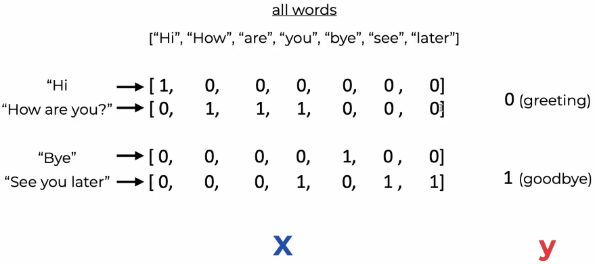
\includegraphics[width=15cm]{img/bagofwords.png}
      \caption{Bag of Words} \label{BagofWords}
      \medskip
      \small
      Usa Bag of Words para separar uma frase em várias palavras. Imagem retirada da Fundamentação Teórica \ref{Fundamentacao}.
   \end{center}
\end{figure}


\begin{lstlisting}[language=Python, caption=Python Bag of Words]
def bag_of_words(tokenized_sentence, words):
    """
    return bag of words array:
    1 para cada palavra conhecida que existe na frase,
    0 caso contrario.


    Exem,plo:


    sentence = ["ola", "como", "esta", "voce"]
    words = ["oi", "ola", "eu", "voce", "tchau",
     "obrigado", "legal"]
    bag   = [  0 ,    1 ,    0 ,   1 ,    0 ,    0 ,      0]
    """
    # stem each word
    sentence_words = [stem(word) for word in tokenized_sentence]
    # initialize bag with 0 for each word
    bag = np.zeros(len(words), dtype=np.float32)
    for idx, w in enumerate(words):
        if w in sentence_words:
            bag[idx] = 1

    return bag

\end{lstlisting}

Durante o processo, também usaremos \textbf{nltkwordtokenize()} que converterá uma única string de sentença em uma lista de palavras. Por exemplo, se você passar \textbf{"Ola, como voce esta?"}, ele retornará \textbf{"ola", "como", "voce", "esta"}.
\textbf{Observação:} Passaremos palavras em minúsculas para o \textbf{Stemmer} para que palavras como Bom e bom (em maiúsculas) não sejam rotuladas como palavras diferentes.

\section[Carregando os dados e Data Cleaning]{Carregando os dados e Data Cleaning}
Usaremos um conjunto de dados chamado  \textbf{intents.json} que tem a estrutura mostrada no campo abaixo. Estaremos limpando esses dados de acordo com as nossas necessidades usando as funções que criamos anteriormente.

\begin{lstlisting}[language=python, caption=Data intents.json]
{
  "intents": [
    {
      "tag": "saudacao",
      "patterns": [
        "Oi",
        "Ei",
        "Como voce esta",
        "Tem alguem ai?",
        "Ola",
        "Bom dia"
      ],
      "responses": [
        "Ei :-)",
        "Ola, obrigado pela visita",
        "Ola, o que posso fazer por voce?",
        "Ola, como posso ajudar?"
      ]
   }
  ]
}


\end{lstlisting}
Agora vamos simplesmente carregar o arquivo json usando a função \textbf{jsonload}.

\begin{lstlisting}[language=Python, caption=Python Carregando dados]
with open('intents.json', 'r') as f:
    intents = json.load(f)
\end{lstlisting}

Para obter as informações corretas, iremos descompactá-las com o seguinte código:

\begin{lstlisting}[language=Python, caption=Python Loop nos dados]
all_words = []
tags = []
xy = []
# loop through each sentence in our intents patterns
for intent in intents['intents']:
    tag = intent['tag']
    # add to tag list
    tags.append(tag)
    for pattern in intent['patterns']:
        # tokenize each word in the sentence
        w = tokenize(pattern)
        # add to our words list
        all_words.extend(w)
        # add to xy pair
        xy.append((w, tag))

\end{lstlisting}
Isso separará todas as tags e palavras em suas listas.
